% !TEX program = xelatex
% !BIB program = bibtex

\documentclass[UTF8,cs4size]{ctexart}

% layout
\usepackage[left=3cm,right=3cm]{geometry}
\linespread{1}
\ctexset{
  section = {
    name = \S
  },
  subsection/name = \S,
  subsubsection/name = \S
}

% page headings
\usepackage{fancyhdr}
\setlength{\headheight}{15.2pt}
\pagestyle{fancy}
\lhead{\leftmark}
\rhead{M201873026 刘一龙}
\cfoot{\thepage}

% url/ref
\usepackage{hyperref}
\hypersetup{
  colorlinks,
  citecolor=black,
  filecolor=black,
  linkcolor=black,
  urlcolor=black,
  pdfauthor={刘一龙},
  pdftitle={迷宫最短路径问题}
}

% vertical centering title page
\usepackage{titling}
\renewcommand\maketitlehooka{\null\mbox{}\vfill}
\renewcommand\maketitlehookd{\vfill\null}

% table of contents
\usepackage{tocloft}
\renewcommand\cftsecfont{\normalfont}
\renewcommand\cftsecpagefont{\normalfont}
\renewcommand{\cftsecleader}{\cftdotfill{\cftsecdotsep}}
\renewcommand\cftsecdotsep{\cftdot}
\renewcommand\cftsubsecdotsep{\cftdot}
\renewcommand{\contentsname}{\hfill\bfseries\Large 目录\hfill}   
\setlength{\cftbeforesecskip}{10pt}

% figures
\usepackage{graphicx}
\graphicspath{figures/}
% \newcommand\figureht{\dimexpr
%   \textheight-3\baselineskip-\parskip-.2em-
%   \abovecaptionskip-\belowcaptionskip\relax}

% tables
\usepackage{caption} 
\captionsetup[table]{skip=10pt}

% math, algorithms, code
\usepackage{amsmath,amssymb,url}
\usepackage{algorithm, algorithmic}
\usepackage{listings}

\lstset{
   extendedchars=true,
   basicstyle=\footnotesize\ttfamily,
   showstringspaces=false,
   showspaces=false,
   numbers=left,
   numberstyle=\footnotesize,
   numbersep=9pt,
   tabsize=2,
   breaklines=true,
   showtabs=false,
   captionpos=b
}

% bibliography
\usepackage[super,square,comma,sort]{natbib} % for \citet and \citep
\renewcommand{\refname}{\S 参考文献}

% appendix
\usepackage{appendix}

\title{\textbf{Assignment1: 迷宫最短路径问题}}
\author{计算机科学与技术学院\\ 硕1801\\ M201873026\\ 刘一龙}
\date{\today}

\begin{document}

\pagenumbering{gobble} % no page number
\maketitle
\newpage
\tableofcontents
\newpage
\pagenumbering{arabic}

\section{问题描述}
定义一个二维数组,表示一个迷宫,其中的 "1" 表示阻挡,"0" 表示可通过:
\begin{equation*}
  \text{int maze}[5][5] =
  \begin{bmatrix}
    0 && 1 && 0 && 0 && 0 \\
    0 && 1 && 0 && 1 && 0 \\
    0 && 0 && 0 && 0 && 0 \\
    0 && 1 && 1 && 1 && 0 \\
    0 && 0 && 0 && 1 && 0
    \label{eq:maze1}
  \end{bmatrix}
\end{equation*}

限制条件:只能横着走或竖着走,不能斜着走。

要求:找出从左上角到右下角的最短路径,写出算法步骤。
\newpage

\section{算法概述}
宽度优先搜索算法(BFS)算法\cite{wiki:Breadth-first_search} 作为遍历树/图的有力工具,可以用于求解迷宫最短路径问题。
进行宽度优先搜索时,当访问至终止顶点处,此时沿搜索路径反向回到起始顶点,这一路径必然是最短路径。具体流程如算法~\ref{alg:bfs}所示。
\begin{algorithm}
  \floatname{algorithm}{算法}
	\renewcommand{\algorithmicrequire}{\textbf{输入:}}
	\renewcommand{\algorithmicensure}{\textbf{输出:}}
	\caption{迷宫最短路径求解算法}
	\label{alg:bfs}
	\begin{algorithmic}[1]
		\REQUIRE 二维数组(表示迷宫)
		\ENSURE 迷宫最短路径
		\STATE $frontiner \leftarrow (0, 0)$
    \STATE $parent[0][0] \leftarrow (0, 0)$
    \STATE $visited[0][0] \leftarrow true$
    \WHILE{$\!frontier.empty()$}
      \STATE $cur \leftarrow frontier.pop()$
      \FOR{$i = 0$ \TO $3$}
        \STATE $next \leftarrow cur.neighbours.directions[i]$
        \IF{$next$ 是终点}
          \STATE $parent[DIM][DIM] \leftarrow cur$ 
          \STATE $\textbf{return } true$
        \ENDIF
        \IF{$next$ 可通且未访问过}
		      \STATE $frontiner \leftarrow next$
          \STATE $parent[next] \leftarrow cur$
		      \STATE $visited[next] \leftarrow true$
        \ENDIF
      \ENDFOR
    \ENDWHILE
    \STATE $\textbf{return } false$
	\end{algorithmic}  
\end{algorithm}
\newpage

\section{实验结果}
利用 C++ 语言实现上述算法后,对三种具有代表性的迷宫进行了测试,即无出路迷宫、单出路迷宫、多出路迷宫。
\subsection{无出路迷宫}
所测迷宫的矩阵表示为:
\begin{equation}
  \text{Matrix } =
  \begin{bmatrix}
    0 && 1 && 0 && 0 && 0 \\
    0 && 1 && 0 && 1 && 0 \\
    0 && 1 && 1 && 1 && 0 \\
    0 && 1 && 1 && 1 && 0 \\
    0 && 0 && 0 && 1 && 0
    \label{eq:maze1}
  \end{bmatrix}
\end{equation}

可以看出,对于迷宫~\eqref{eq:maze1} 从 (0, 0) 至 (4, 4) 没有任何通路,算法输出结果如图~\ref{fig:maze1} 所示,算法正确地求解出了无通路这一结果。
\begin{figure}[htb]
  \centering
    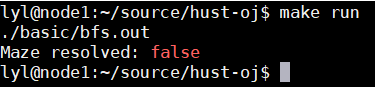
\includegraphics[width=0.7\textwidth,height=3.5cm]{figures/assign1_maze1.png}
  \caption{无出路迷宫算法求解结果}
  \label{fig:maze1}
\end{figure}

\subsection{单出路迷宫}
所测迷宫的矩阵表示为:
\begin{equation}
  \text{Matrix } =
  \begin{bmatrix}
    0 && 1 && 0 && 0 && 0 \\
    0 && 0 && 0 && 1 && 0 \\
    0 && 1 && 1 && 1 && 0 \\
    0 && 1 && 1 && 1 && 0 \\
    0 && 0 && 0 && 1 && 0
    \label{eq:maze2}
  \end{bmatrix}
\end{equation}

可以看出,对于迷宫~\eqref{eq:maze2} 从 (0, 0) 至 (4, 4) 有且仅有一条通路,算法输出结果如图~\ref{fig:maze2} 所示,算法正确地求解出了这一通路。
\begin{figure}[htb]
  \centering
    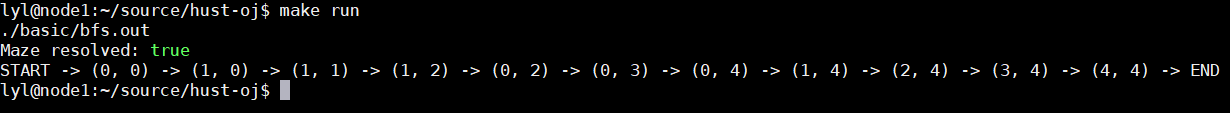
\includegraphics[width=\textwidth,height=3.5cm]{figures/assign1_maze2.png}
  \caption{无出路迷宫算法求解结果}
  \label{fig:maze2}
\end{figure}

\subsection{多出路迷宫}
所测迷宫的矩阵表示为:
\begin{equation}
  \text{Matrix } =
  \begin{bmatrix}
    0 && 1 && 0 && 0 && 0 \\
    0 && 1 && 0 && 1 && 0 \\
    0 && 0 && 0 && 0 && 0 \\
    0 && 1 && 1 && 1 && 0 \\
    0 && 0 && 0 && 1 && 0
    \label{eq:maze3}
  \end{bmatrix}
\end{equation}

可以看出,对于迷宫~\eqref{eq:maze3} 从 (0, 0) 至 (4, 4) 有两条通路,算法输出结果如图~\ref{fig:maze3} 所示,算法正确地求解出了最短通路。
\begin{figure}[htb]
  \centering
    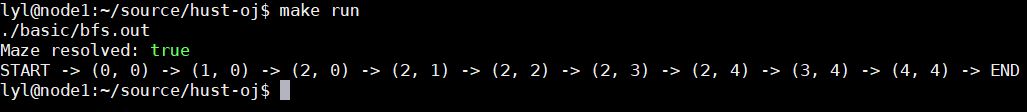
\includegraphics[width=\textwidth,height=3.5cm]{figures/assign1_maze3.png}
  \caption{无出路迷宫算法求解结果}
  \label{fig:maze3}
\end{figure}

\clearpage

\bibliographystyle{unsrt}
\bibliography{bibs/assign1}
\addcontentsline{toc}{section}{\S 参考文献}
\newpage

\begin{appendices}
\section{代码}
\lstinputlisting[language=C++]{code/assign1.cpp}
\end{appendices}

\end{document}
